\documentclass[xcolor=table,english]{beamer}
\usepackage[orientation=portrait,size=a0]{sty/beamerposter}
\usepackage[utf8]{inputenc}
\usepackage{ragged2e}
\usepackage{verbatimbox}
\usepackage[font=small,justification=justified]{caption}
\usepackage{array}
\usepackage{tabularx}

\usepackage[british]{babel} % decent hyphenation, avoiding e.g. anal-ysis
\usepackage[iso]{isodate}
\usepackage{sansmath}
\usepackage{booktabs}
\usepackage{graphicx}
\usepackage{makecell}
\usepackage{minted}
\usepackage{multicol}
\usepackage{siunitx}
\usepackage{subcaption}
%\usepackage{amsmath}
\newcommand{\mathdefault}[1]{#1}
\usepackage[section]{placeins}

% Needs to be loaded after hyperref
\usepackage{cleveref}

\usepackage{import}
% SIunitx customizations detect-all will use the current font for typesetting
\sisetup{per-mode=symbol, detect-all, range-units = single}
\newcommand\SIci[5]{\SI{#1}{#2}, {#3}CI: \SIrange{#4}{#5}{#2}}

% Fix for matplotlib PGF wonkiness which isn't interpreted correctly by pdflatex
\DeclareUnicodeCharacter{2212}{-}


\newcolumntype{Z}{>{\centering\arraybackslash}X} % centered tabularx columns

\newlength{\columnheight}
\setlength{\columnheight}{0.881\textheight}

\mode<presentation>{
	\usepackage{sty/beamerthemeDartmouth}
}

% Set these inputs:
\date{2023-11-10}
\title{
	\href{https://github.com/con/opfvta-reexecution}{
		\Large github.com/con/opfvta-reexecution
	}\\\vspace{.15em}
	Neuroimaging Article Reexecution and Reproduction Assesment System
}
\author{
	Horea-Ioan Ioanas$^{1}$,
	Austin Macdonald$^{1}$,
	Yaroslav O. Halchenko$^{1}$
}
\institute[CON]{$^{1}$Center for Open Neuroscience, Department of Psychological and Brain Sciences, Dartmouth College}

% These need to be inline lest the URL is constructed with whitespace
\newcommand{\myDOI}{10.5281/zenodo.10085170}
\newcommand{\myemail}{horea@dartmouth.edu}

\begin{document}

\begin{frame}
\begin{columns}
	\begin{column}{.42\textwidth}
		\begin{beamercolorbox}[center]{postercolumn}
			\begin{minipage}{.98\textwidth}  % tweaks the width, makes a new \textwidth
				\parbox[t][\columnheight]{\textwidth}{ % must be some better way to set the the height, width and textwidth simultaneously
					\begin{myblock}{Abstract}
						As the scientific world becomes increasingly large and increasingly reliant on automation, reproducibility becomes more and more vital for the successful development of both the scientific community and research technologies.
For most researchers, however, reproducibility remains a nebulous ideal, the benefits of which are considered more theoretical and indirect, than practical and immediate.
In this article we share a reference implementation of an article, which makes the benefits of reproducibility accessible and reusable.
In this article we put forth an explicit reproducibility model, which is both simple and consistently applicable throughout the scientific process, and thus to the work of any scientist.
We proceed to select a set of technologies which strongly facilitate reproducibility, and present to the reader a plethora of reproductions of peer-reviewed scientific work.
While this framework is as all encompassing as possible, we see it thus as an excelent reference implementation which which is reusable across a wide range of topics.

					\end{myblock}\vfill
					\vspace{-0.3em}
					\begin{myblock}{Workflow}
						\vspace{0.5em}
						\begin{figure}
							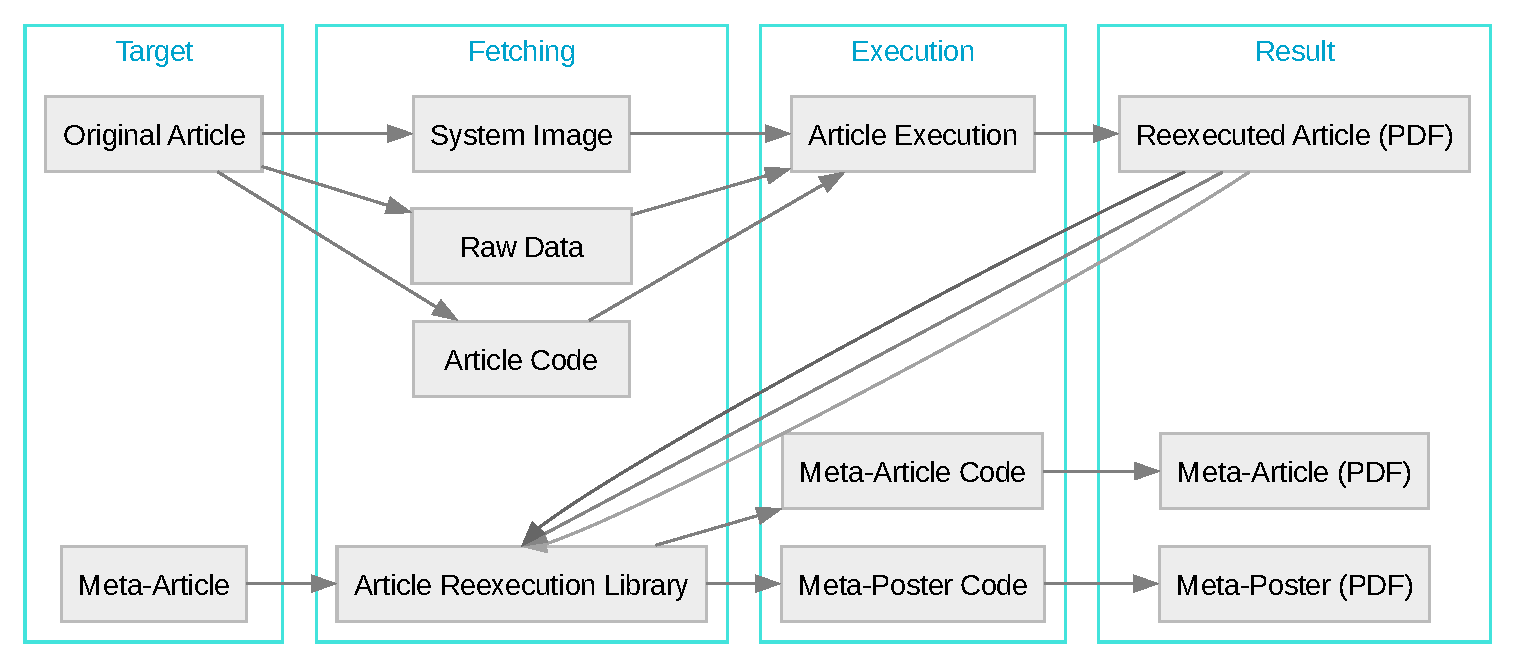
\includegraphics[width=0.99\textwidth]{img/workflow.pdf}
							\caption{
								The reexecution system encompasses both the original article (first target), and the “meta-article” publishing materials (article manuscript, as well as this poster), the latter of which takes user- and developer-submitted reexecution results as an input for the reproduction quality assessment.
							}
						\end{figure}
					\end{myblock}\vfill
					\vspace{-0.3em}
					\begin{myblock}{Topoplogy}
						\vspace{0.5em}
						\begin{figure}
							\captionsetup{width=.9\linewidth}
							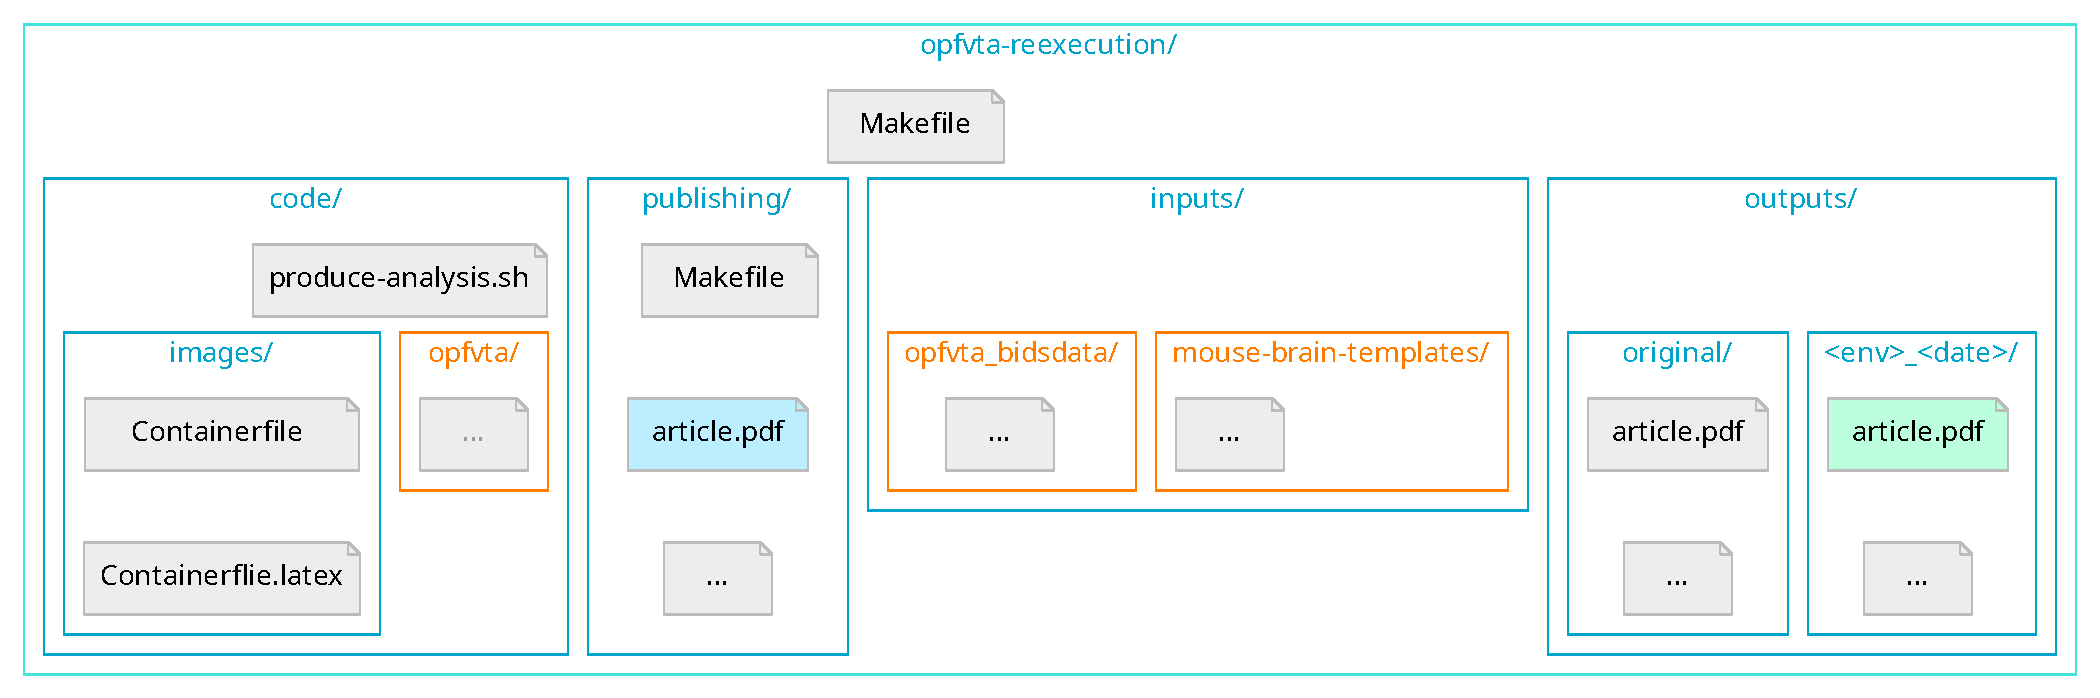
\includegraphics[width=0.99\textwidth]{img/topology.pdf}
							\caption{
								The reexecution workflow is supported by a resource topology in which reexecution code (first box), “meta-article” code (second box), reexecution resources (third box), and the reexecution output record (last box) are separated at the top directory level.
								The figure depicts direcotry trees via nested boxes, with external resources automatically fetched as via the reexecution code being highlighted in orange.
								The green highlighted article represents a sample reexecution output, and the blue hignlighted article represents the manuscript, an analogous output to this poster generated in the same directory.
							}
							\label{fig:workflow}
						\end{figure}
					\end{myblock}\vfill
					\begin{myblock}{Best Practice Guidelines}
						\vspace{0.5em}
						As part of setting up an encompassing reexecution system, we formulate a number of best practices, including:
						\begin{itemize}
							\item \textbf{Errors should be fatal more often than not.}\\
								\colorbox{elg}{\texttt{set -eu}}, prepended to POSIX shell scripts, will ensure that workflows fail when a subcommand does, or when an encountered variable is undefined.
							%\item \textbf{Avoid assuming or hard-coding absolute paths to resources.}\\
							\item \textbf{Avoid assuming a directory context for execution.}\\
								%\colorbox{elg}{\texttt{cd \textquotedbl\$(dirname \textquotedbl\$0\textquotedbl)\textquotedbl}}, prepended to POSIX shell scripts, will ensure that in complex workflows scripts can operate relative to their location directory context and not the execution context.
								\colorbox{elg}{\texttt{cd "\$(dirname "\$0")"}}, prepended to POSIX shell scripts, will ensure that in complex workflows scripts can operate relative to their location directory context and not the execution context.
							\item \textbf{Workflow granularity greatly benefits efficiency.}\\
								While the underlying execution system of the target article, RepSeP \cite{repsep} separates data analysis into two distinct (voxel-space “low iteration” and top-level “high iteration”) steps, further granularity can benefit debugging, particularly in container environments.
							%\item Container image size should be kept small.
							\item \textbf{Resources should be bundled into a DataLad superdataset.}\\
								Resource bundling, with usage of submodules for external resources (as seen in \cref{fig:workflow}) allows management of required resources via Git and associated technologies, such as DataLad \cite{datalad} — this is known as the YODA principle \cite{yoda}.
							%\item Containers should fit the scope of the underlying workflow steps.
							%\item Do not write debug-relevant data inside the container
							%\item Parameterize scratch directories
							\item \textbf{Dependency versions inside container environments should be frozen as soon as feasible.}\\
								This is best accomplished via a package manager which uses version tracking for its software provision index; in Gentoo Linux, used here on account of broad provision of neuroscience packages \cite{ng}, this can be done via: \colorbox{elg}{\texttt{cd /.../myrepo; git fetch origin \$myhash; git checkout \$myhash}}.
						\end{itemize}
					\end{myblock}\vfill
					\begin{myblock}{References}
						\vspace{0.5em}
						\begin{minipage}{.3\textwidth}
							\begin{figure}
								
\includegraphics[width=0.9\textwidth]{img/qr.eps}
							\end{figure}
						\end{minipage}
						\begin{minipage}{.69\textwidth}
							\scriptsize
                                                        \bibliographystyle{ieeetr}
                                                        \bibliography{bib}
						\end{minipage}
					\end{myblock}\vfill
		}\end{minipage}\end{beamercolorbox}
	\end{column}
	\begin{column}{.59\textwidth}
		\begin{beamercolorbox}[center]{postercolumn}
			\begin{minipage}{.98\textwidth} % tweaks the width, makes a new \textwidth
				\parbox[t][\columnheight]{\textwidth}{ % must be some better way to set the the height, width and textwidth simultaneously
					\begin{myblock}{Reproduction Assessment Showcase}
						\vspace{-0.45em}
						\begin{minipage}{.58\textwidth}
						\begin{figure}
							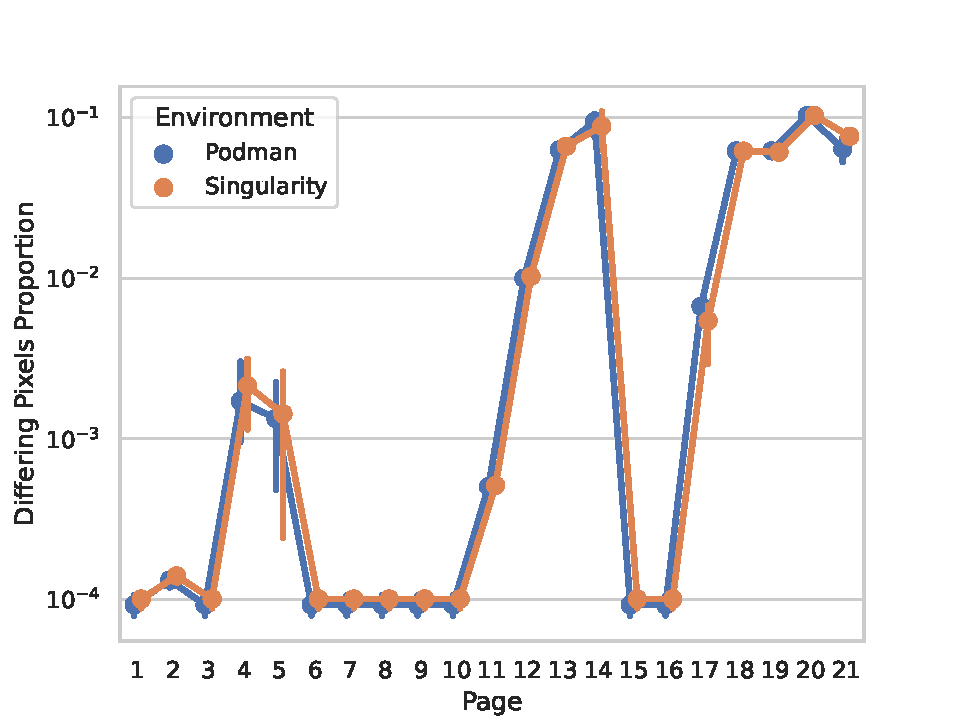
\includegraphics[width=0.95\textwidth]{img/diff_pages.pdf}
							\vspace{0.2em}
							\caption{
								Page-wise pixel difference comparison across multiple reexecutions in different environments indicates consistency of variability in both extent and location.
							}
							\label{fig:ras_s}
						\end{figure}
						\begin{figure}
							\fbox{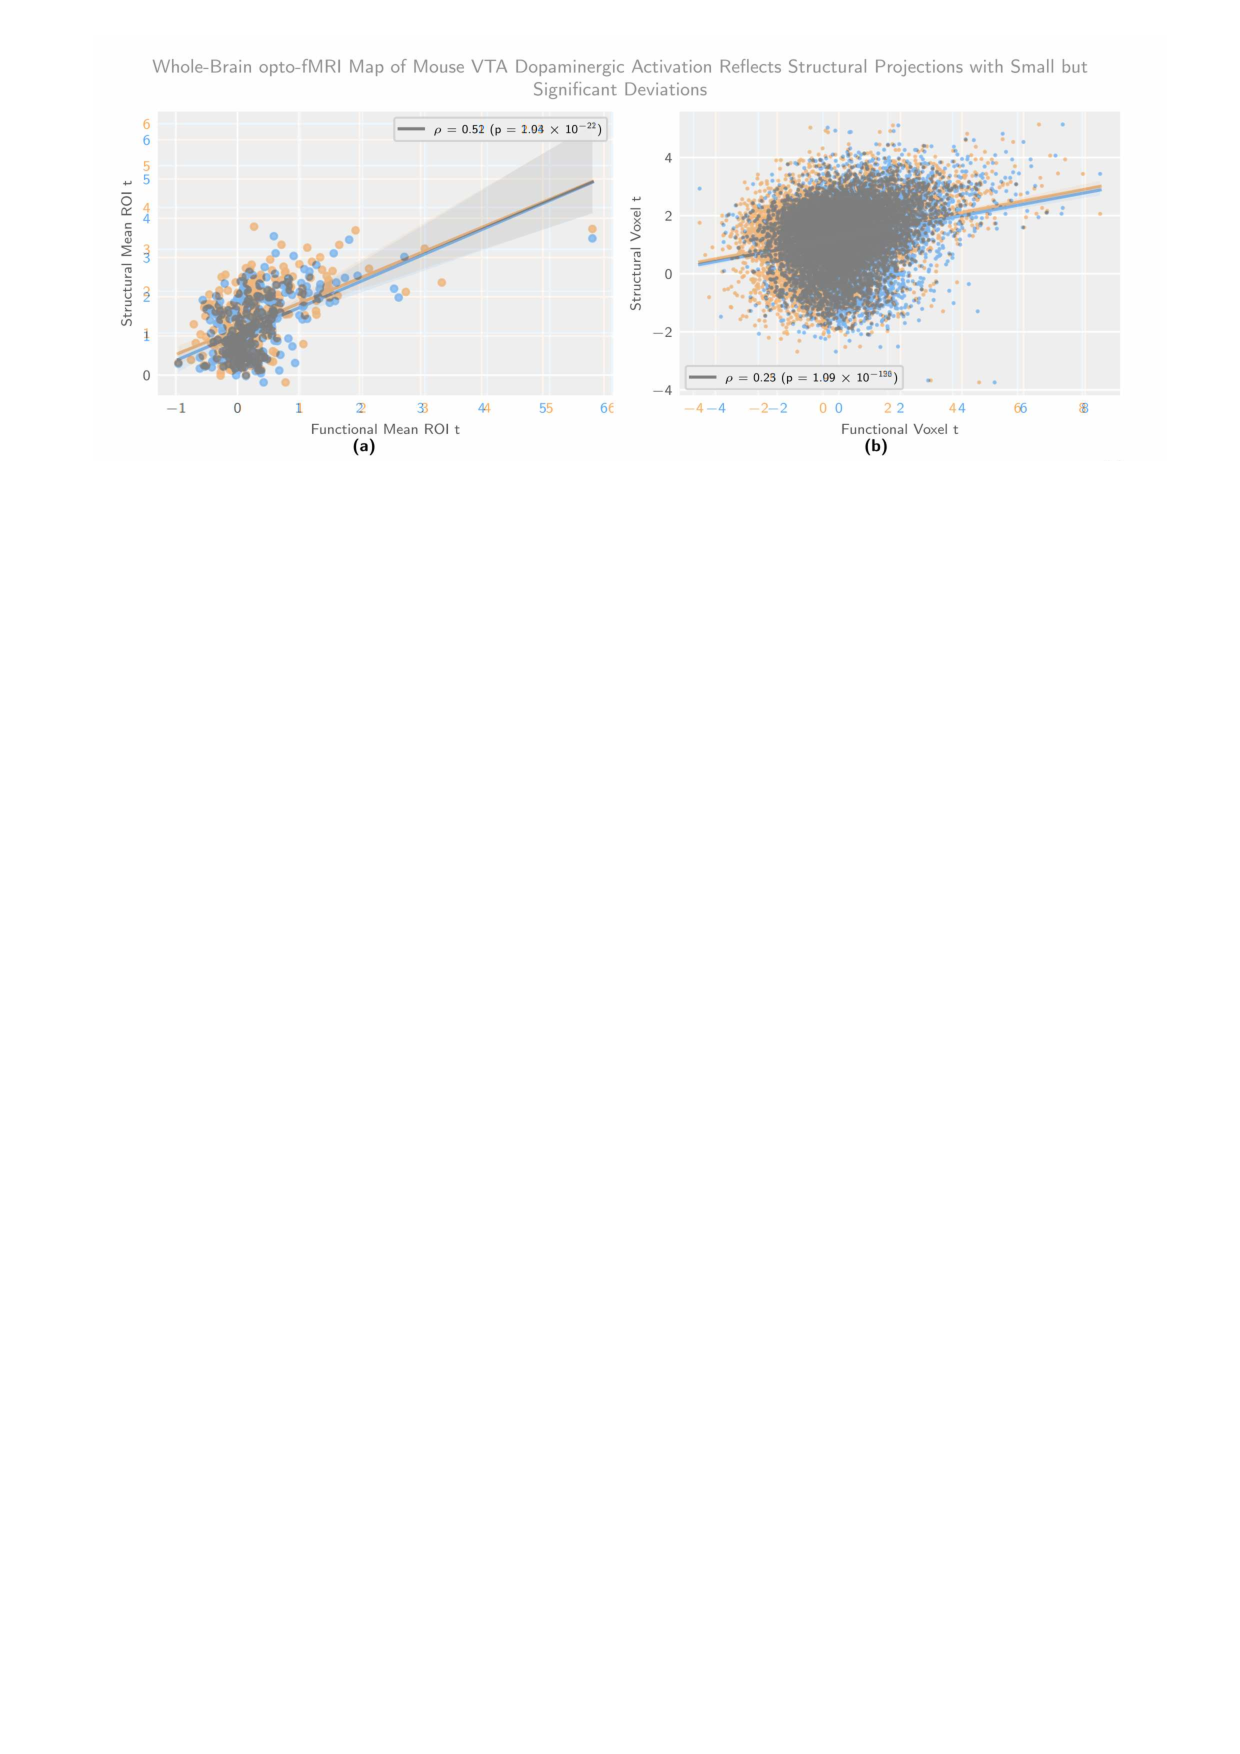
\includegraphics[width=0.9\textwidth]{img/diff_fig.pdf}}
							\vspace{0.2em}
							\caption{
								One notable source of variability are data plots, where it can be observed that even as data points vary to an almost full extent, statistical summaries can remain constant.
							}
						\end{figure}
						\end{minipage}
						\hfill
						\begin{minipage}{.38\textwidth}
						\vspace{1.3em}
						\begin{figure}
							\fbox{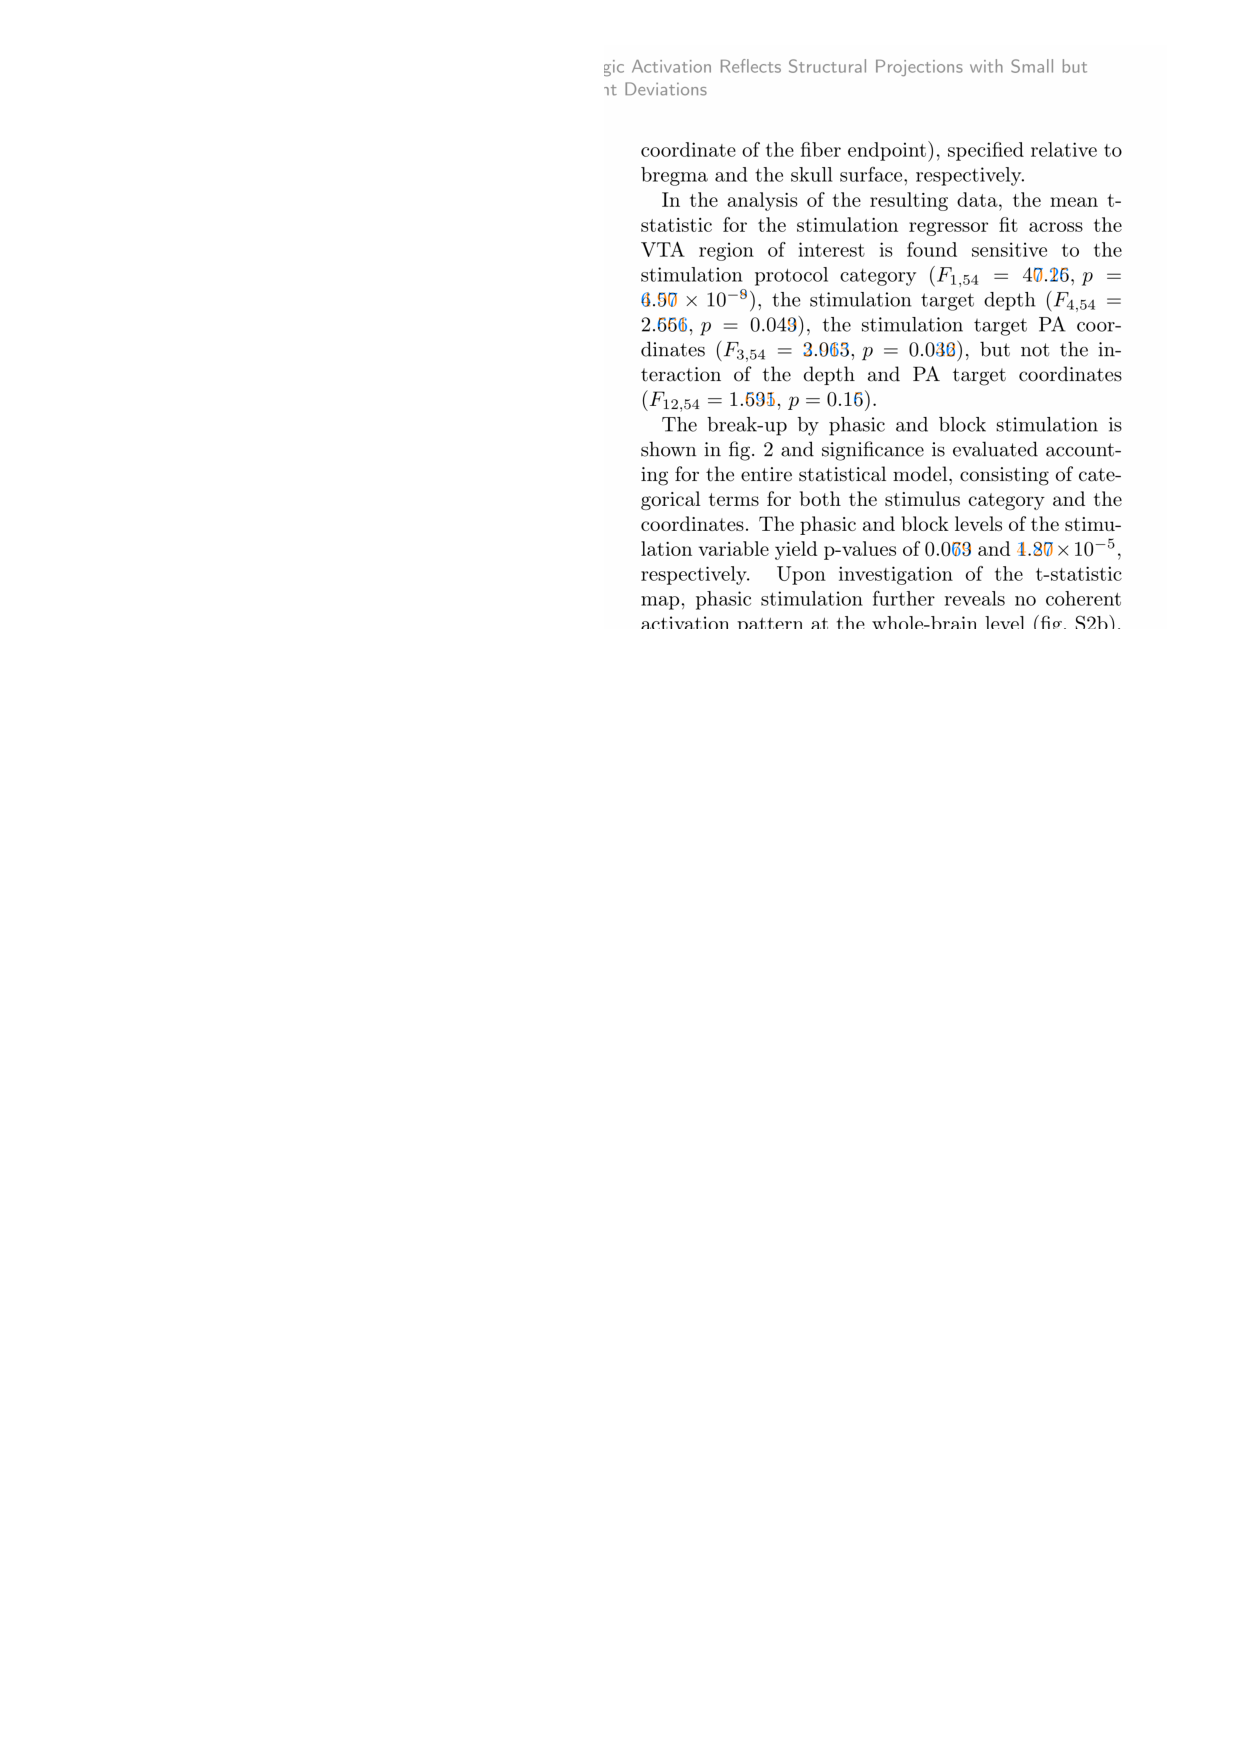
\includegraphics[width=0.9\textwidth]{img/diff_text.pdf}}
							\vspace{0.5em}
							\caption{
								Text differences in statistical summaries account for a small proportion of voxel differences, but can remain well-localized instead of spreading via test shift if statistical summaries are appropriately trimmed down to a constant length.
							}
						\end{figure}
						\begin{figure}
							\fbox{
\includegraphics[width=0.9\textwidth]{img/diff_date.pdf}}
							\vspace{0.5em}
							\caption{
								A good litmus test for monitoring differences (accounting for the baseline difference in \cref{fig:ras_s}) is the datestamp of the reexecution, which should always be expected to differ from the manuscript.
							}
						\end{figure}
						\end{minipage}
					\end{myblock}\vfill
					\begin{myblock}{Full Document Comparison}
						\vspace{0.25em}
						Reproduction assessment is based on \textit{full} document “diffs”.
						The following figures are excerpts, with tinted highlighting (blue for the original manuscript, and orange for reexecution result).
						First row pages exemplify inline statistical differences and second row pages exemplify figure differences.
						Differing sections are highlighted with a red left-hand marking.\\
						\vspace{0.75em}
						\fbox{\includegraphics[page=4,scale=1.04]{img/marked_paperdiff_singularity_20230908122618.pdf}}
						\fbox{\includegraphics[page=5,scale=1.04]{img/marked_paperdiff_singularity_20230908122618.pdf}}
						\\
						\vspace{.3em}
						\fbox{\includegraphics[page=13,scale=1.04]{img/marked_paperdiff_singularity_20230908122618.pdf}}
						\fbox{\includegraphics[page=14,scale=1.04]{img/marked_paperdiff_singularity_20230908122618.pdf}}
					\end{myblock}\vfill
		}\end{minipage}\end{beamercolorbox}
	\end{column}
\end{columns}
\end{frame}
\end{document}
